\documentclass[border=10pt]{standalone}
\usepackage{verbatim}
\usepackage{pgfplots}
\pgfplotsset{compat=1.14}

% stars_count = 512;
% max_time = 2.5
% steps = {0.1, 0.1 / 8, 0.1 / (8 * 8), 0.1 / (8 * 8 * 8), 0.1 / (8 * 8 * 8 * 8)};

\begin{document}

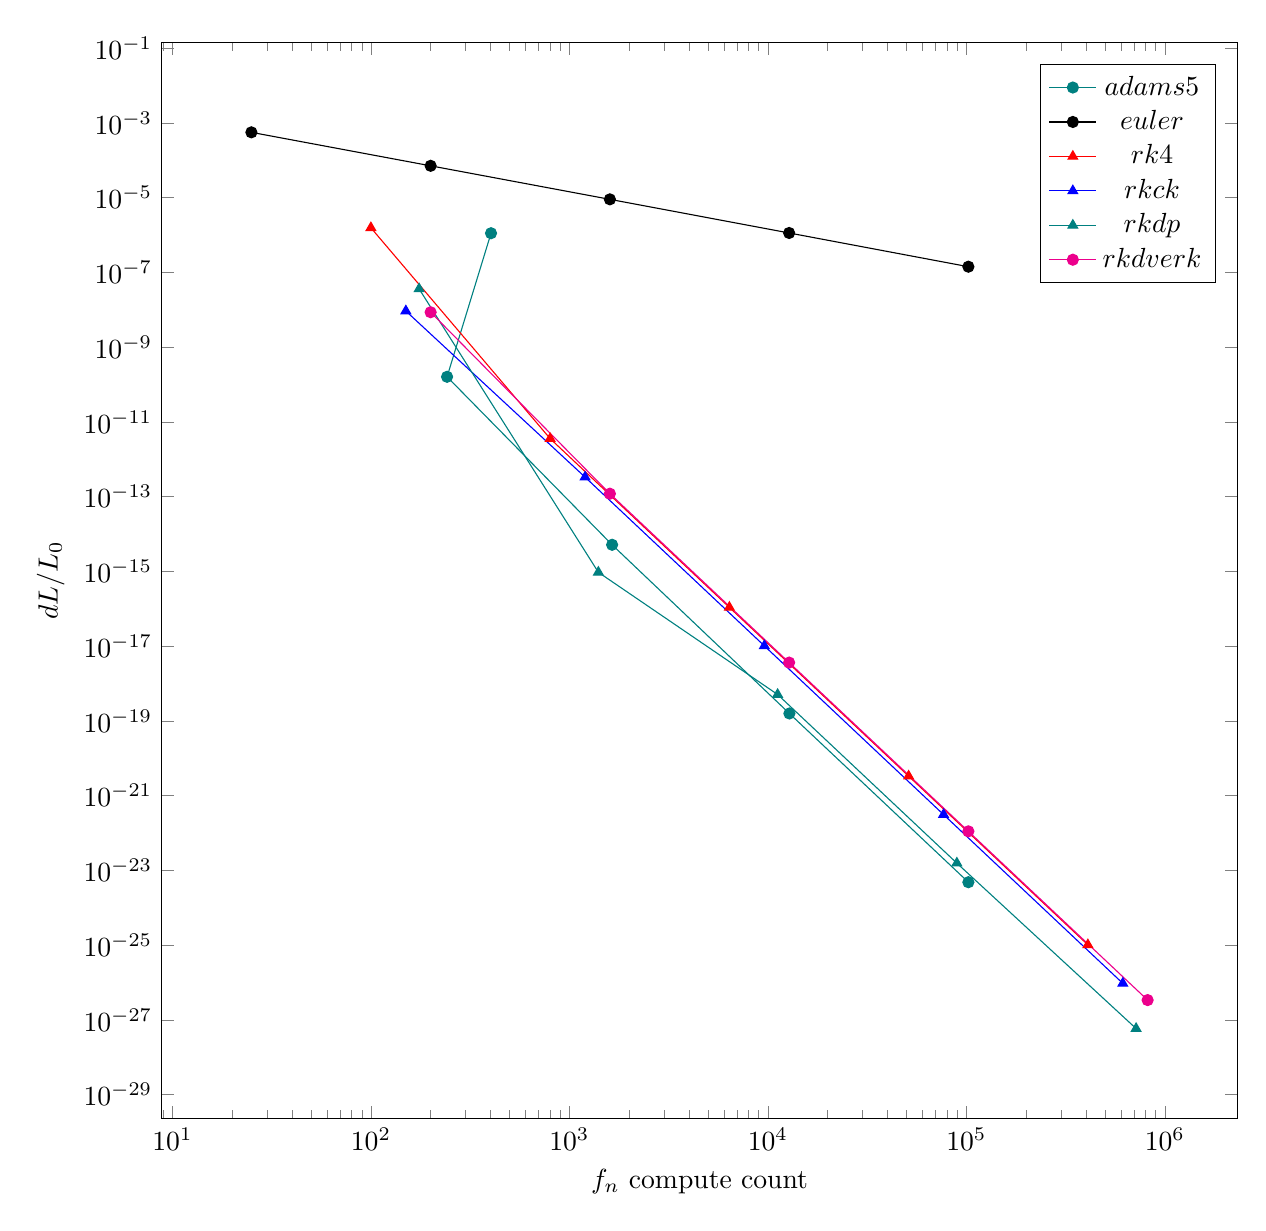
\begin{tikzpicture}
\begin{loglogaxis}[
    height=6in,
    width=6in,
    xlabel=$f_n$ compute count,
    ylabel=$dL/L_0$
]
\addplot [teal,mark=*,solid] coordinates { (403, 1.117e-06) (242, 1.607e-10) (1642, 5.139e-15) (1.284e+04, 1.574e-19) (1.024e+05, 4.805e-24) };
\addplot [black,mark=*,solid] coordinates { (25, 0.0005593) (200, 7.107e-05) (1600, 9.009e-06) (1.28e+04, 1.134e-06) (1.024e+05, 1.419e-07) };
\addplot [red,mark=triangle*,solid] coordinates { (100, 1.562e-06) (800, 3.566e-12) (6400, 1.086e-16) (5.12e+04, 3.313e-21) (4.096e+05, 1.014e-25) };
\addplot [blue,mark=triangle*,solid] coordinates { (150, 9.265e-09) (1200, 3.32e-13) (9600, 1.016e-17) (7.68e+04, 3.1e-22) (6.144e+05, 9.444e-27) };
\addplot [teal,mark=triangle*,solid] coordinates { (175, 3.617e-08) (1400, 9.442e-16) (1.12e+04, 5.069e-19) (8.96e+04, 1.557e-23) (7.168e+05, 5.832e-28) };
\addplot [magenta,mark=*,solid] coordinates { (200, 8.583e-09) (1600, 1.197e-13) (1.28e+04, 3.622e-18) (1.024e+05, 1.105e-22) (8.192e+05, 3.372e-27) };
\legend{$adams5$,$euler$,$rk4$,$rkck$,$rkdp$,$rkdverk$};
\end{loglogaxis}
\end{tikzpicture}

\end{document}
